\documentclass[12pt]{article}
\usepackage[style=apa]{biblatex}
\DeclareLanguageMapping{english}{english-apa} % Resolve labelyearlabelmonthlabelday errors.
\AtEveryBibitem{\clearfield{note}} % Clear note fields.
\usepackage{listings}
\usepackage{enumitem}
\usepackage{lipsum}
\usepackage[symbol]{footmisc}
\usepackage{graphicx}
\usepackage[capposition=top]{floatrow}
\usepackage{listings}
\usepackage{hyperref}
\usepackage{bibentry}
\usepackage[letterpaper, left=1in,top=1in,right=1in,bottom=1in]{geometry}
\usepackage{setspace}
\usepackage{epstopdf}
\usepackage{amssymb}
\usepackage{lineno}
\usepackage{wrapfig}
\usepackage{amsmath}
\usepackage{array}
\usepackage{color,soul}
\usepackage{tabularx}
\usepackage{rotating}
\usepackage{lscape}
\usepackage{subcaption}
\usepackage{longtable}
\usepackage{siunitx}
\usepackage{appendix}
\usepackage{pdfpages}
\usepackage{titlesec}
\usepackage{mfirstuc}
\usepackage{multirow}
\usepackage{threeparttable}
\usepackage{color,soul}
\usepackage{todonotes}

\renewcommand{\baselinestretch}{1.5}
\renewcommand{\thefootnote}{\fnsymbol{footnote}}
\bibliography{../reference/classification.bib}
\bibliography{../reference/algorithms/ml_algorithms.bib}
\setcounter{tocdepth}{2}


\title{\textbf{\capitalisewords{Classification of nonprofit organizations: A supervised machine-learning approach}}}
\author{%
\textsc{Ji Ma and Isha Kanani} \thanks{J.M.: maji@austin.utexas.edu, LBJ School of Public Affairs and RGK Center for Philanthropy and Community Service; I.K.: ishakanani@utexas.edu, School of Information.} \\[1ex] % Your name \thanks{}
\normalsize University of Texas at Austin \\ % Your institution
% \normalsize {Email: maji@austin.utexas.edu} \\ % Your email address
}


\date{\today} % Leave empty to omit a date \today

%----------------------------------------------------------------------------------------

\begin{document}

\maketitle

\begin{abstract}
\noindent This research note reports the use of supervised machine-learning algorithms in classifying the nonprofit organizations in the United States. Mission statements and project descriptions are collected from the 990 forms as text data, and classifications using National Taxonomy of Exempt Entities are collected from the National Center for Charitable Statistics at the Urban Institute. Three text classification algorithms are experimented: Na\"ive Bayes, Random Forest, and Neural Network. The Neural Network classification achieves the best results with an average accuracy of 9*.9\% (standard deviation **), recall *** (standard deviation **), and precision *** (SD **). An open-source Python package \textit{npocat} is developed and shared using the trained algorithms. Future projects are discussed.

% The National Taxonomy of Exempt Entities (NTEE) has been used for classifying the nonprofit organizations in the United States for several decades. However, major countries in the world do not have a classification system for the nonprofit sector. This paper achieves three major goals: 1) devising a machine learning model which can classify the nonprofits using mission statements, 2) inventing a functional classification system which can be applied to different countries, 3) test the accuracy of the model and classification system. We first created a classification system cross different countries by matching existing standards, then compiled the training and testing datasets for China (data from China Foundation Center and Research Infrastructure of Chinese Foundations), United Kingdom (data from ****), and United States (data from National Center for Charitable Statistics and Internal Revenue Service). We finally test the accuracy of major text classification algorithms using country-specific training datasets and a pooled dataset. Implications and limitations are discussed.
\end{abstract}
\clearpage

\listoftodos
\clearpage

\section{Introduction}

Although the voluntary and philanthropic organizations have long been existent for numerous centuries, the so-called ``nonprofit sector'' was only coined in the 1970s by scholars, policy makers, and nonprofit practitioners. A major reason for assembling the diverse organizations as a conceptual whole is to legitimize the existence of these organizations and the benefits these organizations receive \parencites[54-55]{HallHistoricalOverviewPhilanthropy2006}{BarmanClassificatoryStrugglesNonprofit2013}. From Durkheim's \citeyear{DurkheimElementaryFormsReligious2012} perspective, the order and structure of a society can be reflected by a classification system. The National Taxonomy of Exempt Entities (NTEE) developed by the National Center for Charitable Statistics (NCCS), the most widely used classification system, is one of the efforts legitimizing the existence of nonprofit sector \parencite{Hodgkinsonnewresearchplanning1991,HodgkinsonMappingnonprofitsector1990}. As \textcite[105]{BarmanClassificatoryStrugglesNonprofit2013} cite \textcite[601]{ClarkeSimpleTechnologyComplex1996}: ``The ways in which different entities (people, animals, plants, diseases, etc.) are organized into classificatory groups reveal something of the social, cultural, symbolic, and political contexts within which classifications occur.''

The development of NTEE classifications can date back to the 1980s \parencite[8-9, 11]{HodgkinsonMappingnonprofitsector1990}. In 1982, NCCS assembled a team of experts working on creating a taxonomy for nonprofit organizations. The first draft of the taxonomy, entitled ``National Taxonomy of Exempt Entities'' (NTEE), came out in 1986 and published in 1987. In the early 1990s, NCCS had classified nearly one million nonprofits using NTEE. In 1995, the Internal Revenue Service (IRS) adopted the NTEE coding system, took over the tasks of assigning and maintaining the classifications, and started to release the Business Master File with NTEE codes \parencite{USInternalRevenueServiceExemptOrganizationsBusiness2014,USInternalRevenueServiceIRSStaticFiles2013}.

Two agencies took the task of assigning NTEE codes: NCCS and IRS. Before 1995, NCCS coded nonprofits according to the program descriptions in Part III and VIII of Form 990, supplemented with information from Form 1023 (``Application for Recognition of Exemption'') and additional research \parencite[16]{NationalCenterforCharitableStatisticsGuideUsingNCCS2006}. After 1995, IRS began to issue ``new exempt organizations an NTEE code as part of the determination process,'' and ``the determination specialist assigns an NTEE code to each organization exempt under I.R.C. \S 501(a) as part of the process of closing a case when the organization is recognized as tax-exempt'' \parencite[1]{USInternalRevenueServiceIRSStaticFiles2013}.

The NTEE classifications has been used for numerous practical and academic purposes. For example, it provides a framework on which the social and economic activities of nonprofits can be mapped and compared with other types of organizations in a society \parencite[e.g.,][]{RoegerNonprofitSectorIts2015}. It can also serve as an analytical tool for measuring the organizational capacity in different service domains and inform the practitioners and policymakers in decision-making \parencite{Hodgkinsonnewresearchplanning1991}. Scholars also use NTEE codes for sampling purposes \parencite[e.g.,][]{OktenDeterminantsdonationsprivate2000,CarmanEvaluationCapacityNonprofit2010} or as independent variables \parencite{SloanEffectsNonprofitAccountability2009}. The invention of NTEE also provides a fundamental necessity for comparative international research, facilitating the study of ``global civil society'' \parencite{VakilConfrontingclassificationproblem1997,Salamonsearchnonprofitsector1992,Salamoninternationalclassificationnonprofit1996,HodgkinsonMappingnonprofitsector1990}.

The NTEE classification system, although one of the best we have, still has several major drawbacks. First, because it only assign one major category code to an organization, it cannot accurately describe a nonprofit organization's programs which are usually diverse and across several domains \parencite[303]{GronbjergUsingNTEEclassify1994}. Although another classification system assigning purpose codes to programs was developed \parencite{LampkinIntroducingNonprofitProgram2001}, it is not widely used \hl{(why?)}. Second, the assignment of NTEE codes is not complete because it is ``based on an assessment of program descriptions contained in Parts 3 and 8 of the Form 990'' and ``program descriptions were only available for some organizations'' \parencite[16]{NationalCenterforCharitableStatisticsGuideUsingNCCS2006}. A recent study found the number of organizations in Washington State with a specific NTEE code could be significantly increased if the mission statements were used for coding \parencite{FyallNTEECodesOpportunities2018}. Third, NTEE codes are static but nonprofit organizations' activities may change over time. Recoding existent NTEE assignments is extremely onerous, and this may be one of the reason that IRS does not have a procedure by which the nonprofits can request the change of their NTEE codes \parencite{USInternalRevenueServiceIRSStaticFiles2013}.
\todo[inline]{NTEE limitations: \textcite{Salamonsearchnonprofitsector1992}.}

\todo[inline]{Contribution of this study.}

% By using supervised machine-learning techniques, this study advanced the NTEE classification system from the following perspective: 1) A series of datasets for training models was developed, 2) the accuracy and efficiency of popular text-classification algorithms were compared, 3) existent empirical studies were replicated to test the validity of our machine-learning approach. According to the results of experimentation, validation, and replication, the combination of \hl{\textit{ABC} algorithm} and trained datasets produced the best results.

\section{Method}

\subsection{Working with Texts and Research Workflow}

The classification of texts is a typical task of automatic content analysis, and three types of methods are common to this task: dictionary, supervised, and unsupervised methods \parencite[268-269]{GrimmerTextDataPromise2013}. The dictionary methods use a predefined dictionary of words to classifying the texts. Although accurate, this approach is not capable to deal with the variations and contexts of language. An improved solution is to use supervised methods which are computer algorithms that can ``learn'' the linguistic patters in a dataset classified by human coders. Unlike the dictionary and supervised methods which require predefined categories of interest, unsupervised methods can discover linguistic patters in texts without inputting any knowledge of classification. However, the validity of unsupervised methods is a serious challenge because the classifications returned may not be theoretically meaningful. This study employs supervised methods to make the use of existing classifications and human-coded records and deal with linguistic variations and contexts. 

\todo[inline]{Research workflow.}
\begin{figure}
	\centering
	\caption{\textsc{Research workflow}} \label{fig:workflow}
	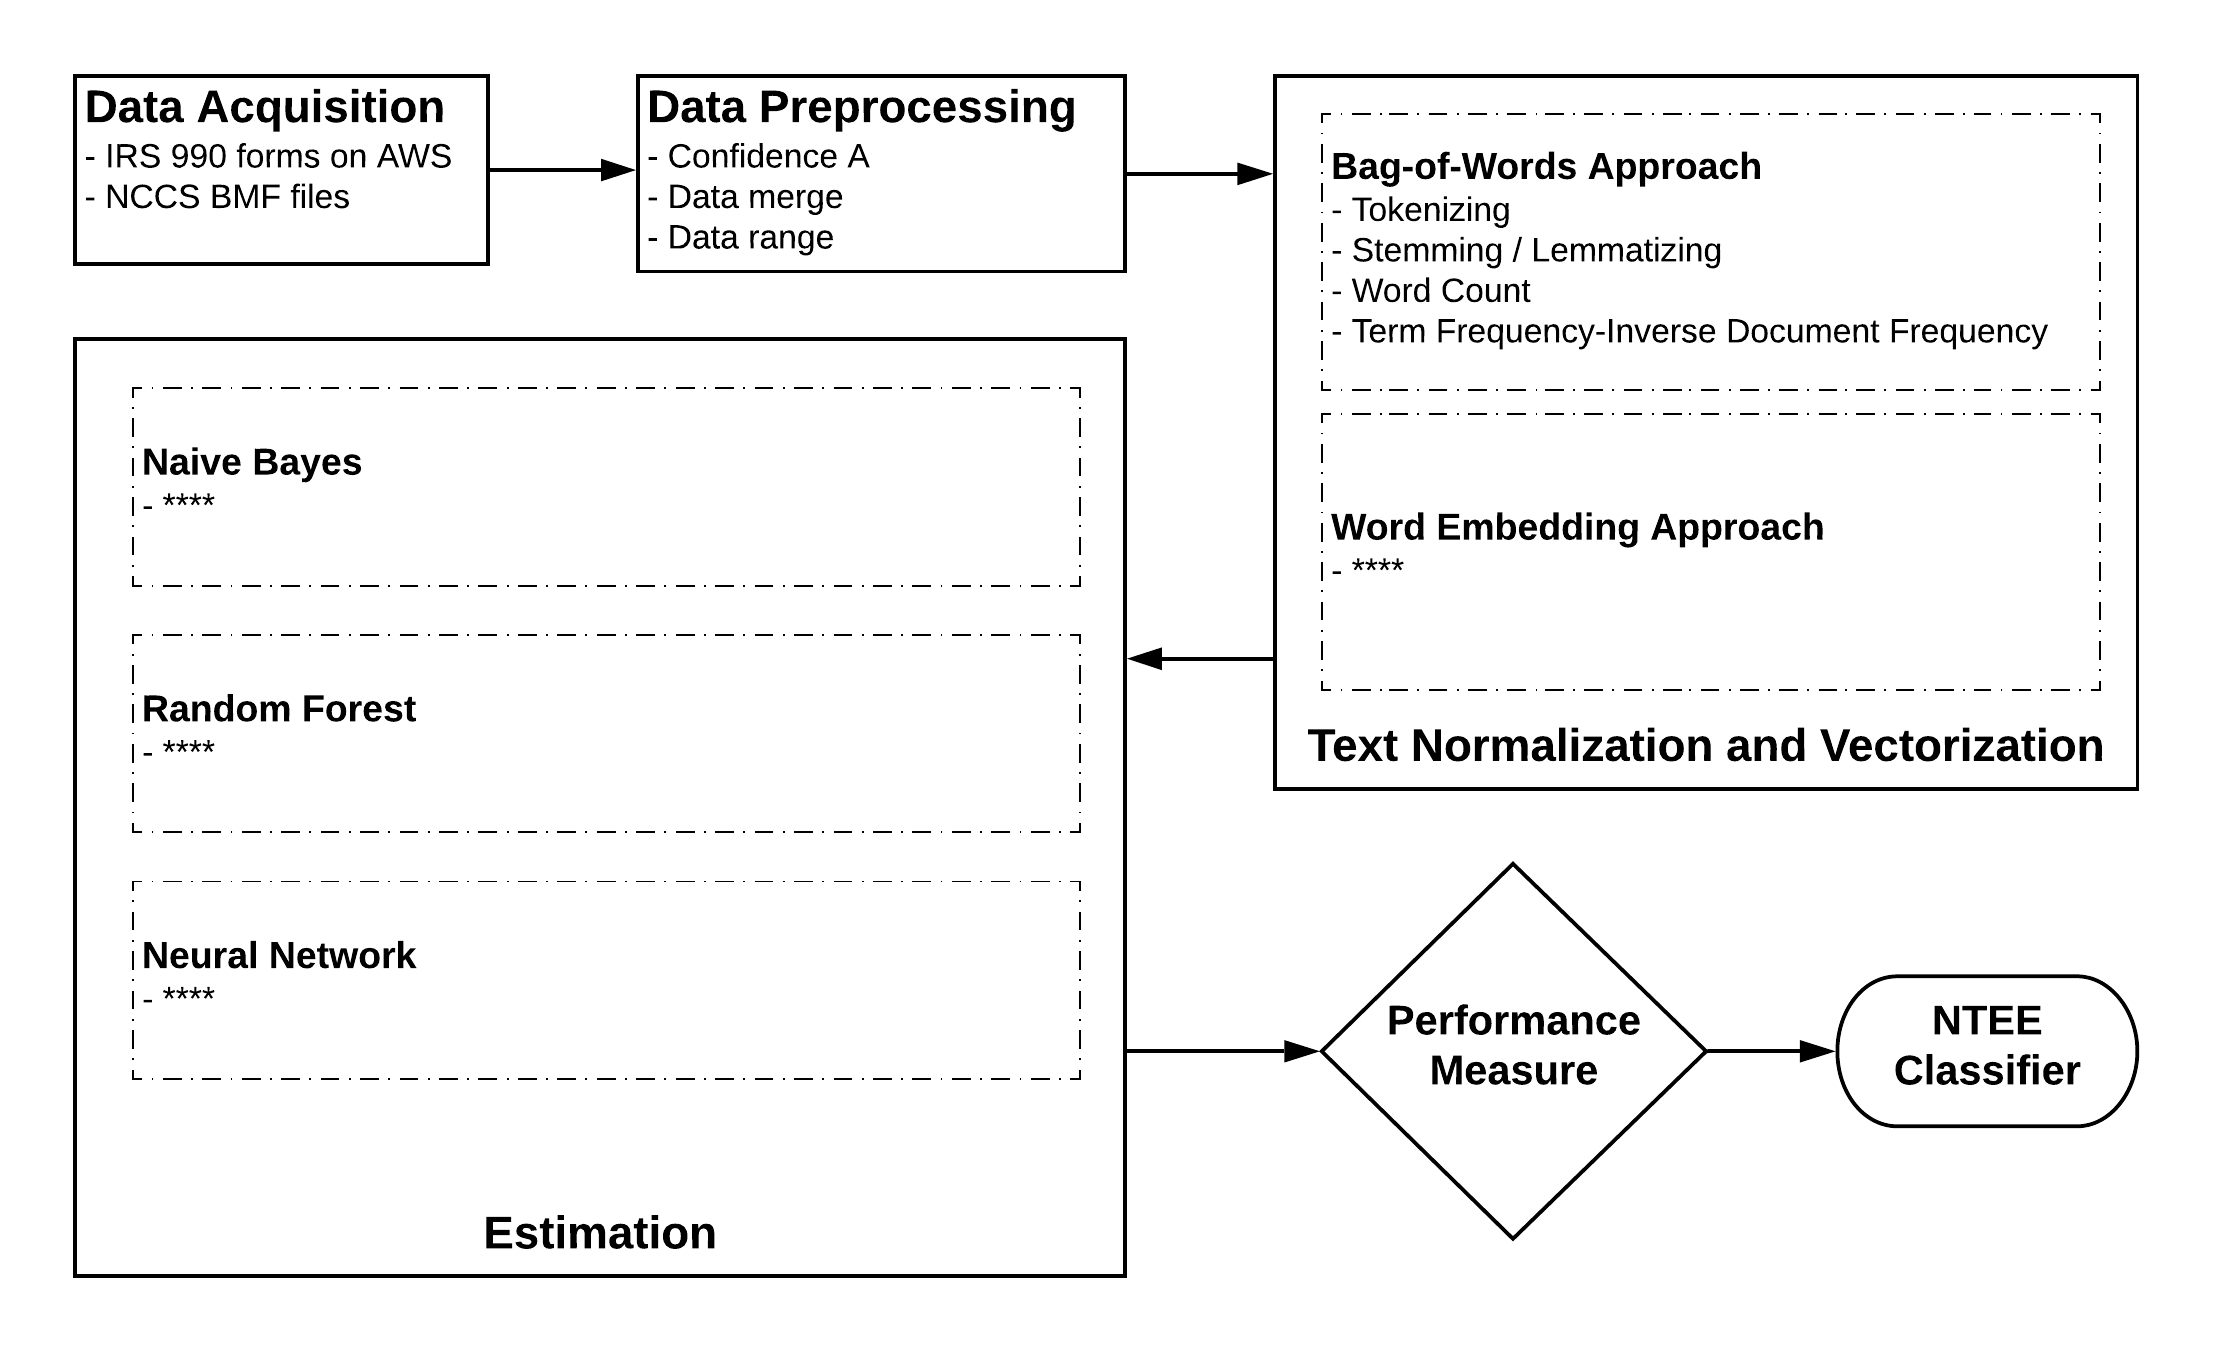
\includegraphics[width=1\textwidth]{paper/tbl_fig/NTEE-workflow.png}
\end{figure}


\subsection{Data Acquisition}

There are two types of datasets for supervised text classification: training dataset and testing dataset. Both datasets are collections of text records that have been classified by human coders. The machine-learning algorithms can ``learn'' the linguistic patters from the training dataset and then classify the records in testing dataset using the patters learned. The results generated by algorithms can be compared with those coded by human coders, and ultimate goal is to use trained models to replace human. The quality of training dataset is decisive because it must be a representative sample of the whole corpus. The training dataset can be generated by randomly sampling the whole corpus, but a better strategy is proportional sampling according to the distribution of classification scheme \parencite[278]{GrimmerTextDataPromise2013}.

\subsubsection{Text Data}

Text records are collected from three forms: 990, 990-EZ, and 990-PF, supplemented with program descriptions from Schedule O. Form 990 (Return of Organization Exempt From Income Tax) is submitted by most of the nonprofit organizations. For smaller organizations with ``gross receipts of less than \$200,000 and total assets of less than \$500,000 at the end of their tax year'' \parencite[1]{USInternalRevenueService2017InstructionsForm2018}, they can file Form 990-EZ (Short Form Return of Organization Exempt From Income Tax), a shorter version of Form 990. Form 990-PF (Return of Private Foundation) is only for private foundations. Different forms generally have two types of texts describing the organizational activities: overall mission statement and specific program description. Table \ref{text_loc} summarizes the specific locations of the text fields in different forms.

\begin{table}[]
    \centering
    \begin{tabularx}{\textwidth}{r|X|X}
         & Mission & Program \\
         \hline
         990 & Part I, Line 1; Part III, Line 1 & Part III, Line 4; Part VIII, Line 2a-e, Line 11a-c; Schedule O \\
         990-EZ & Part III & Part III, Line 28-30; Schedule O \\
         990-PF & -- & Part IX-A; Part XVI-B \\
    \end{tabularx}
    \caption{Locations of text fields in different forms.} \label{text_loc}
    \label{tab:my_label}
\end{table}

\subsubsection{Classification Data}
BMF file. 

\subsection{Data Preprocessing}

\subsubsection{Sampling}
\todo[inline]{Why and how to do the bootstrap sampling \parencite[596]{Erceg-HurnModernrobuststatistical2008}.}
A confidence level of A, B, or C is assigned to indicate the accuracy of classification, ``A confidence level of A, for example, indicates that there is at least a 90 percent probability that the major group classification is correct'' \parencite[16]{NationalCenterforCharitableStatisticsGuideUsingNCCS2006}. From 2014 to 2016, 56.12\% records are classified at A level, 37.32\% at B level, and 6.56\% at C level. For training purposes, we only include records at confidence level A in the training dataset. But we include all the records at different confidence levels in the testing dataset, expecting the performance of ML algorithms should decrease as the confidence level goes from A to C.

\todo[inline]{Time range of data records; descriptive statistics of data records.}

Figure \ref{fig:NTEE_dist} shows the proportions of NTEE major categories from 1989 to 2015 ... 
\todo[inline]{Figures or tables describing the patterns of datasets.}

\subsection{Text Normalization}
\todo[inline]{why need normalization.}

\subsubsection{Tokenization} \todo[inline]{Explain.}

\subsubsection{Stemming and Lemmatization} \todo[inline]{Explain.}

\subsection{Text Vectorization}
\todo[inline]{why need vectorization.}

\subsubsection{Bag-of-Words Approach}

In the context of text classification: Na\"ive Bayes classifier needs a set of features as an input, hence we need to provide our text in the form of a set that consists of words from the text. This representation is called bag-of-words \parencites{Jurafsky:2009:SLP:1214993}, which consists of all important words from the text, and the number of times each word occurs in the text. Since the input is a set of words, all the words are considered to be mutually independent of each other. This means that the order in which the words occur in the text is not considered in this classification, i.e. the input for ``Manchester City beat Barcelona'' and ``Barcelona beat Manchester City'' will be the same bag-of-words.

In the training data set, each ``text'' is converted to a bag-of-words where the mission statement is converted into the set of words and given as an input. Along with the input, the output class ``label'' is also provided for the training purpose. The classifier links each input set with its corresponding output class and trains itself. For testing purpose, the classifier is given a bag-of-words as an input and asked to predict the class with the highest probability for given set of words.

\textit{Count Vector.} \todo[inline]{Explain.}

\textit{Term Frequency-Inverse Document Frequency (TF-IDF).} \todo[inline]{Explain.}

\subsubsection{Word Embedding Approach}
\todo[inline]{1. the cons of bag-of-words. 2. The advantage of using word embedding. 3. The word embedding used in this study.}

% \begin{figure}
% \caption{Draft to be modified}
% \label{classification_algo}
% \centering
% 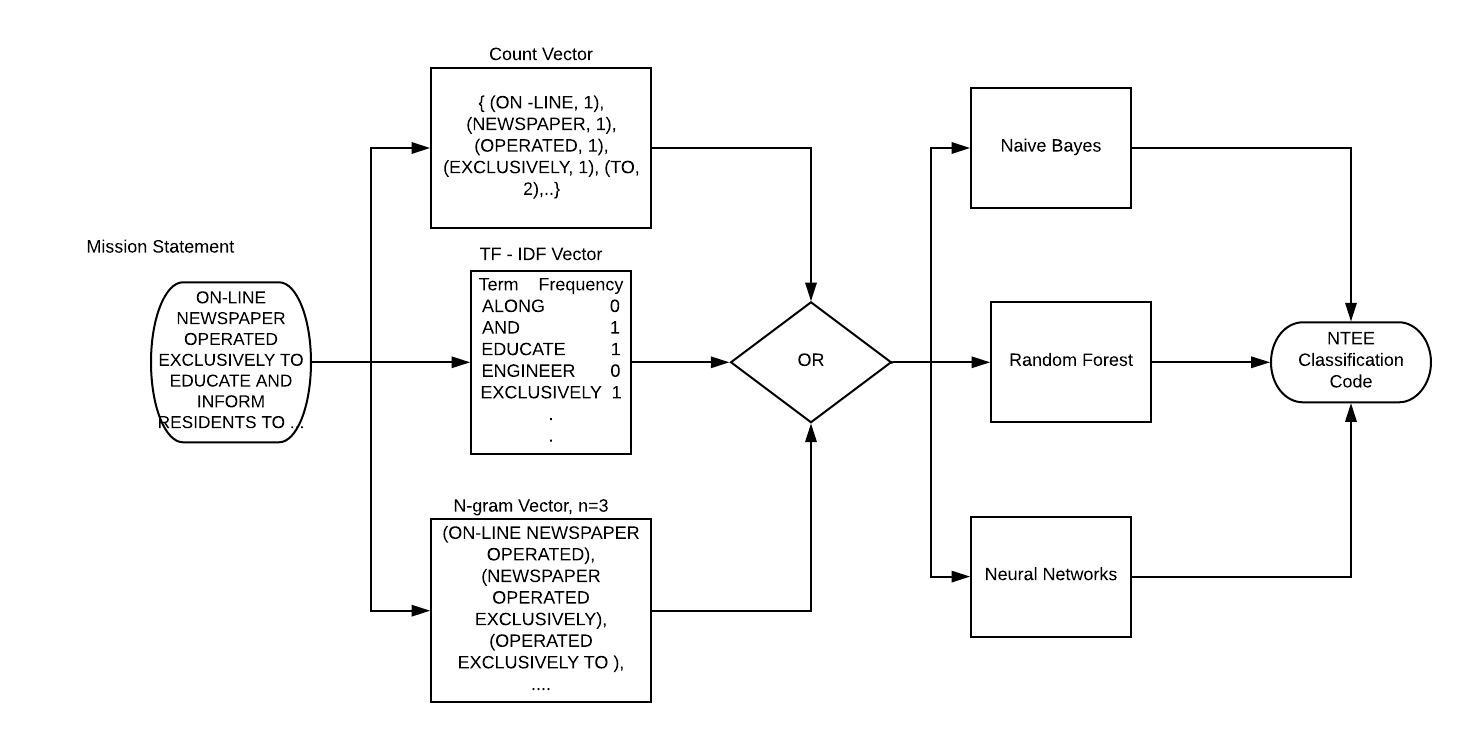
\includegraphics[width=\textwidth]{reference/algorithms/classification_algo.jpeg}
% \end{figure}


\subsection{Estimation}

This study uses three supervised machine-learning classification algorithms: Na\"ive Bayes, Random Forest, and Neural Network.

\subsubsection{Na\"ive Bayes Classification}

Na\"ive Bayes classification is primarily built on Baye\'s theorem \parencites[34]{upton2014dictionary}. Eq. \ref{bayes} calcuate the probability that organization $i$ belonging to a $NTEE$ classification (e.g., ``A'', arts, culture, and humanities), given its text collection $TXT$ defined in Table \ref{text_loc} (e.g., mission statement and program descriptions). 

\begin{equation} \label{bayes}
 P(NTEE_i \mid TXT_i) = \frac{P(TXT_i \mid NTEE_i) \, P(NTEE_i)}{P(TXT_i)} 
\end{equation}

Na\"ive Bayes classifier is one of the simplest classifiers to learn and implement among all machine learning algorithms. It is built on simple conditional probability principles and uses less computational resources. The classifier works well even with a small dataset. It assumes all features (i.e., the $TXT$ in our case) are independent, which is not always true in real-life scenarios \parencites{lewis1998naive}. So the classifier may not perform well on dependent features.

\subsubsection{Random Forest Classification}

\todo[inline]{Revise this section, use NB section as a reference.}

Random forest algorithm is implemented by developing multiple prediction models. Each model in this algorithm is trained by different data, and then all of these models are asked to predict for the same record. A prediction class that is elected by most of these small algorithms is given as the prediction result by random forest algorithm. It uses the word forest because each small algorithm trained is a decision tree \parencites[83]{quinlan1986induction}. A decision tree represents a set of questions that usually has Yes/No answers. Each decision tree is trained on a different training set \parencites[124]{breiman1996bagging}. For example, if our training set S consists of n records, and we have total of m decision trees in our random forest, our training set is divided into m different sets, one training set for each tree, each set consisting of n/m randomly selected records. Since each tree is trained on different set, when a record is given for prediction, each tree predicts the class independent of other tree. In total of m class predictions are collected, and the class which has the highest occurrence in the prediction results is given as the final predicted class by the random forest algorithm. 

While providing training set, a decision tree learns how to classify any organization into NTEE codes based on whether a word occurs in the mission statement or not. While words from a mission statement is given for the testing purpose, a decision tree uses the words it has from training purpose, examines whether each word is present in the word set given or not, and predicts the final NTEE code.

Pros and Cons: Random Forest classifier trains each tree independently with unique training set, which strengthens the performance. The visual interpretation of the classifier is not easy.

\subsubsection{Neural Network Classification}

\todo[inline]{Finish this section.}

Neural Network Classification is built on the concepts of a neuron structure of the human mind. Each neuron in the network is connected to few other neurons of the network by a numerical value called ``weight''. The neurons process records each one in turn, and learn by looking at their classification (i.e., NTEE code in this case) with the known previous NTEE codes of records. With every new record the neurons learn, they update the connection value ``weight'' to update the model \parencites[163]{collobert2008unified}. After the network is done processing each record of the training set, it has final weights for each connection between two neurons. When a testing set is provided, the neurons use the final weights to predict the class (NTEE code), which is most likely to contain such test set.

Pros and Cons of Neural Networks: Neural Networks algorithm beats many other machine learning algorithms in most cases. However, the model only works well when the data is in significant amount. Along with the large size of data, this classification method also consumes a high computation power to train the network. One of the biggest disadvantages of Neural Networks is its ``Black Box Nature'' \parencites{benitez1997artificial}.

\subsection{Measuring Algorithm Performance}

The performance of a classification algorithm can be measured by {accuracy}, {precision}, and {recall}. The \textit{accuracy} measures the percentage of correctly classified organizations as showed in Eq. \ref{accuracy}, where $i$ is one of the three classification algorithms (i.e., NB, RF, and NN), $Org^{correct}$ is the number of organizations correctly classified by the algorithm $i$, and $Org^{total}$ is the total organizations to be classified. For example, $Accuracy^{RF}=0.6$ indicates that, when RF classifies an organization, the chance of getting right is 60\%.

\begin{equation} \label{accuracy}
    Accuracy^i=\frac{Org^{correct}}{Org^{total}}
\end{equation}

The \textit{precision} and \textit{recall} measures the performance of a classifier on a specific category. In Eq. \ref{precision}, $k$ is one of the NTEE codes, $Org^{correct}_{k}$ is the number of organizations correctly classified as $k$ by algorithm $i$, and ${Org^{i}_{k}}$ is the number of organizations classified as $k$ by algorithm $i$. $Org^{correct}_{k}$ will always be smaller than or equal to ${Org^{i}_{k}}$ because ML algorithms can hardly predict everything right. For example, $Precision^{NN}_{B}=0.75$ indicates that 75\% of all the organizations classified as ``education'' by the NN algorithm are correct.

\begin{equation} \label{precision}
    Precision^{i}_{k}=\frac{Org^{correct}_{k}}{Org^{i}_{k}}
\end{equation}

Given a human coder labels an organization as category \textit{k}, the \textit{recall} measures the chance the classifier \textit{i} also identifies the organization as \textit{k}. In Eq. \ref{recall}, $Org^{hum}_{k}$ is the number of organizations that has been classified as $k$ by human coders. For example, $Recall^{NN}_{B}=0.80$ denotes that 80\% of the organizations classified as ``education'' by human coders are correctly identified by the NN algorithm.

\begin{equation} \label{recall}
    Recall^{i}_{k}=\frac{Org^{correct}_{k}}{Org^{hum}_{k}}
\end{equation}


\section{Results}

\subsection{Confusion Matrix}

% \subsection{Applying the International Nonprofit Classification System: Descriptive analysis}
% \subsection{Applying the International Nonprofit Classification System: Replication of empirical studies}


\singlespacing
\sloppy
\printbibliography

\end{document}